\documentclass{fefu_thesis/cls/fefu}

\usepackage{float}
\usepackage{caption}
\usepackage{subcaption}
\usepackage{hyperref}

\author{Терехов Д.Е.}
\setschool{ШКОЛА ЕСТЕСТВЕННЫХ НАУК ДВФУ}
\setgroup{Б8403а}

\begin{document}
    \tableofcontents
    \pagebreak
    \begin{abstract}
        В данной работе представлены два эффективных алгоритма: генерация текстурного меша с последующим упрощением и упаковка полигональных текстур в атлас. Оба алгоритма работают с полигонами следующих типов: невыпуклые, полигоны с дырами, полигоны, состоящие из нескольких контуров.

        \textit{Ключевые слова: генерация меша, упрощение полигонов, упаковка в контейнеры.}
    \end{abstract}
    \pagebreak
    {\centering\section*{Введение}}
    Целью работы является решение задач упрощения полигонов и упаковки, которые играют важную роль в таких прикладных областях, как компьютерная графика, GIS системы, промышленность и т.д. Решение этой задачи также опирается на прикладную область: компьютерную графику, а именно автоматическую генерацию текстурного меша с последующей упаковкой полигональных текстур в текстурные атласы.

    Упаковка в текстурные атласы это один из этапов подготовки ассетов-текстур для оптимального использования: маленькие текстуры становятся частью большого изображения -- текстурного атласа. Это позволяет минимизировать затраты по памяти, а также уменьшить количество вызовов на отрисовку. Полигонизация текстур позволяет уменьшить количество вызовов фрагментного шейдера, путем минимизации площади пустых пикселей, входящих в меш. Также это позволяет упаковать больше текстур в атлас, т.к. в полигональном виде они занимают меньшую площадь.

    К сожалению, нет открытых программных пакетов или статей, которые решают поставленные задачи. Все программные пакеты являются проприетарными, а известные статьи решают данные задачи в очень упрощенном виде. Это и послужило мотивацией для проведение исследований и создания новых алгоритмов.

    В разделе "Раз" более подробно описывается проблема, подлежащая решению, дается обзор теоретических положений и практических подходов к решению поставленных задач.

    В разделе "Два" предлагается теоретическое решение, формируются критерии оценки эффективности алгоритмов, обоснование их корректности. Также приводится описание вспомогательных и основных алгоритмов.

    В разделе "Три" описывается применение результатов исследования в реальном проекте -- игровом движке с открытым исходным кодом <<Citrus>>.

    \section*{Глоссарий}
    \section{Задачи упрощения полигонов и упаковки в контейнеры}

    Целью работы является решение задач упрощения полигонов и упаковки, которые играют важную роль в таких прикладных областях, как компьютерная графика, GIS системы, промышленность и т.д. Решение этой задачи также опирается на прикладную область: компьютерную графику, а именно автоматическую генерацию текстурного меша с последующей упаковкой полигональных текстур в текстурные атласы.

    \subsection{Генерация текстурного меша}

    Полигональный меш (полигональная сетка) -- это совокупность вершин, рёбер и граней, которые определяют форму многогранного объекта в трёхмерной компьютерной графике и объёмном моделировании. В двумерной компьютерной графике меши используются для вершинной и скелетной анимации.

    \begin{figure}[H]
        \centering
        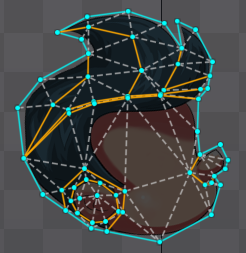
\includegraphics[scale=0.5]{images/spine_mesh.png}
        \caption{2D меш}
    \end{figure}

    Для того, чтобы отрисовать изображение на экране, необходимо пройти через графический конвейер. Обязательными и важнейшими этапами графического конвейера являются исполнение вершинного и фрагментного шейдеров, которые запускаются для каждой вершины и каждого фрагмента (пикселя) соответственно. После вызова фрагментного шейдера полученный цвет фрагмента смешивается с цветом фрагмента в буфере кадра. Многие изображения содержат огромное количество прозрачных пикселей. Вызов фрагментного шейдера для таких пикселей часто является бессмысленным, так как прозрачных пиксель при смешивании никак не повлияет на цвет на экране.
    Эти размышления приводят к одному из способов оптимизации: создание полигонального меша для изображения таким образом, чтобы минимизировать число вершин и пустых пикселей, занимаемых площадью меша.

    \begin{figure}[H]
        \centering
        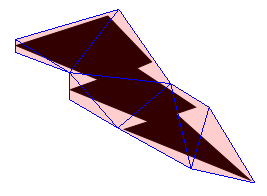
\includegraphics{images/Thunder_approx.png}
        \caption{Полигональный меш с 10 вершинами}
    \end{figure}

    Для GIS систем разработали множество алгоритмов упрощения кривой: алгоритм Ramer–Douglas–Peucker\cite{Ramer}\cite{DouglasPeucker}, алгоритм радиального расстояния\cite{PolylineSimplification}, алгоритм Visvalingam–Whyatt\cite{VisvalingamWhyatt}, упрощение Opheim\cite{Opheim} и Lang\cite{Lang}, алгоритм Zhao–Saalfeld\cite{ZhaoSaalfeld}, алгоритм Reumann-Witkam\cite{ReumannWitkam}.

    Однако в данной работе задача упрощения полигонов применяется в контексте текстурного меша. Ключевыми отличиями данной прикладной задачи от общей является минимизация не только количества вершин, но и площади прозрачных пикселей (или добавочной площади), а также ограничение, которое не позволяет нарушать границы исходных полигонов (контур изображения). Описанные выше алгоритмы можно адаптировать, чтобы они соответствовали ограничению. К сожалению, данные алгоритмы совсем не рассчитаны на минимизацию добавочной площади, а также часто приходят в тупиковую ситуацию, когда все ещё требует уменьшить количество вершин, но возможных трансформаций не существует. Решение данных проблем привело к созданию алгоритма упрощения множества простых полигонов с дырками.

    \subsection{Упаковка текстур в атласы}

    Упаковка в текстурные атласы это один из этапов подготовки ассетов-текстур для оптимального использования: маленькие текстуры становятся частью большого изображения -- текстурного атласа. Под­текстуры отображаются на объект, используя UV ­преобразование, при этом координаты в атласе задают, какую часть изображения нужно использовать. В приложениях нередко используется множество маленьких текстур, причём переключение с одной текстуры на другую является относительно медленным процессом. Поэтому в подобных ситуациях целесообразно применение одного большого изображения вместо множества маленьких. Также текстурные атласы помогают сэкономить память при помощи полигональной упаковки и\textbackslash или алгоритмов сжатия.

    Задача упаковки в контейнеры -- NP-трудная комбинаторная задача. Задача заключается в упаковке объектов предопределённой формы в конечное число контейнеров предопределённой формы таким способом, чтобы число использованных контейнеров было наименьшим или количество или объём объектов (которые упаковывают) были наибольшими. В данной работе предлагается решение 2D irregular bin packing problem, т.е. упаковка полигональных объектов в прямоугольные контейнеры.

    Для упаковки прямоугольных объектов существует множество эвристических алгоритмов\cite{ThousandWayToPackBin}, которые хорошо показывают себя на практике. В области упаковки полигонов существуют различные подходы.

    No-fit polygon\cite{NofitPolygon}\cite{NofitPolygon2} -- это конструкция, которая определяет все положения, которые могут принимать 2 произвольных многоугольника относительно друг друга так, чтобы они соприкасались, но не перекрывались. Часто методы на основе no-fit polygon используют для решения задачи раскроя на производстве, где форма вырезаемых объектов несложная и заранее известна.

    Swarm intelligence (роевой интеллект) -- метод оптимизации, который описывает коллективное поведение децентрализованной самоорганизующейся системы: колонии светлячков\cite{FireFly}, муравьев\cite{AntColony}, пчел\cite{PlayrixArticle}, particle swarm optimization\cite{PSO}.

    Генетический алгоритм\cite{JAKOBS1996165} -- это эвристический алгоритм поиска, используемый для решения задач оптимизации и моделирования путём случайного подбора, комбинирования и вариации искомых параметров с использованием механизмов, аналогичных естественному отбору в природе.

    К сожалению, результаты прочитанных статей не удовлетворяют нужды упаковки текстур в атласы, поэтому данная работа предлагает собственную реализацию Memetic algorithm -- расширение генетического алгоритма, которое использует локальный поиск для уменьшения вероятности преждевременной сходимости. Разработанный алгоритм способен упаковывать изображения, на которых находятся множество разрозненных объектов с дырами.
    \newpage
    \bibliographystyle{ugost2008ls}
    \bibliography{references}
\end{document}
